\subsection{Detection of a spherical object in the sub-surface}
\label{Sec:SphereInSubsurface}
\begin{enumerate}[label=(\alph*)]
  \item Consider a spherical object with radius $R$ located at depth $z$ below the surface, and a gravimeter that is moved along the surface across the anomaly (Fig.\ref{Fig:SphereInSubsurface}). Derive an analytical expression for the expected \textit{vertical} anomaly $g_z$ as a function of the lateral distance $x$ and depth $z$. Calculate the maximum anomalies that you would expect for some realistic settings (e.g., a limestone cave.)

  \item Use a piece of paper or a software of your choice (e.g., Excel, SciDAVis, Matlab, Python) and visualize the expected vertical gravity anomaly for a specific setting as a function of lateral distance $x$. Show how this profile changes as you vary the depth of the object. 

  \item Sometimes results in the gravity method are expressed in \textit{mGal} with 1 Gal = 0.01 m s$^{-2}$. Transfer your results to those units and post a picture of your graph in the forum.

  \item We now investigate how we can estimate the depth of the object from an anomaly as derived in (a,b). For this you have to derive an expression that links the half-width of the anomaly (i.e. $g_z = \frac{1}{2}g_{z,max}$ for $x=x_{1/2}$) to the depth $z$ of the object. Derive this relationship which has the form $z = c x_{1/2}$. Why is such a relationship be useful?
\end{enumerate}

\begin{figure}
\centering
\begin{minipage}[c]{0.5\textwidth}
\begin{center}
    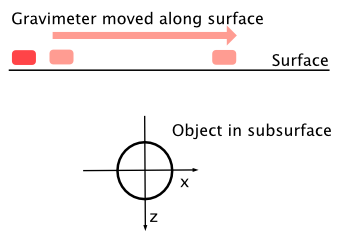
\includegraphics[width=\textwidth]{Figures/Gravimetry/Gravimetry01_SphereSketch.png}
\end{center}
\caption{Sketch for problem \ref{Sec:SphereInSubsurface}. It is easiest to choose a coordinate system with the origin inside the subsurface object.}
\label{Fig:SphereInSubsurface}
\end{minipage}
\end{figure}

\ifanswers
    \begin{tcolorbox}[enhanced jigsaw,breakable,pad at break*=1mm,
    colback=blue!5!white,colframe=babyblueeyes,title=Solutions]
     \begin{center}
       
\includegraphics[width=0.5\textwidth]{Figures/Gravimetry/Gravimetry01_SphereSketchSolutions.png}
    \end{center}
    \textbf{(a)} Because we have a spherical object, we can use the shell theorem and treat it as a point mass. The gravitational force exhibited by the sphere is:
    $$
    \vec{g} = -G\frac{M}{r^2}\hat{r}
    $$
    where $\hat{r}$ is the unit vector pointing from the center of mass to our gravimeter at the surface. The minus sign makes sure that the force is attractive (and not repulsive). The mass anomaly $M$ formulated in a relative sense of the sphere is given by:
    $$
    M = \frac{4}{3}\pi R^3 \Delta \rho
    $$
    At distance $x$ the distance to the sphere is $r=\sqrt{x^2+z^2}$. The gravimeter only measures the vertical component of $\vec{g}$:
    $$
    g_z = -|\vec{g}|\cos\phi = -|\vec{g}|\frac{z}{r}
    $$
  
    which brings us to:
    \begin{eqnarray*}
    g_z &=& -\frac{4}{3}\pi R^3 \Delta \rho \frac{G}{r^2} \frac{z}{r} \\
        &=& -\frac{4}{3}\pi R^3 \Delta \rho \frac{G}{r^3} z \\
        &=& -\frac{4}{3}\pi R^3 \Delta \rho G \frac{z}{(x^2+z^2)^\frac{3}{2}}
    \end{eqnarray*}
    We will encounter the maximum value of the anomaly at $x = 0$ (directly above the target):
    $$
    g_{z,max} = \frac{4}{3}\pi R^3 \Delta \rho G \frac{1}{z^2}
    $$
    which for the limestone cave example is approximately -0.35 mGal (see below).
    

    \textbf{(b, c)}
    \lstinputlisting[language=matlab]{../../Src/Exercises/Gravimetry/Gravimetry01_SphereVisualization.m}
    \begin{center}
        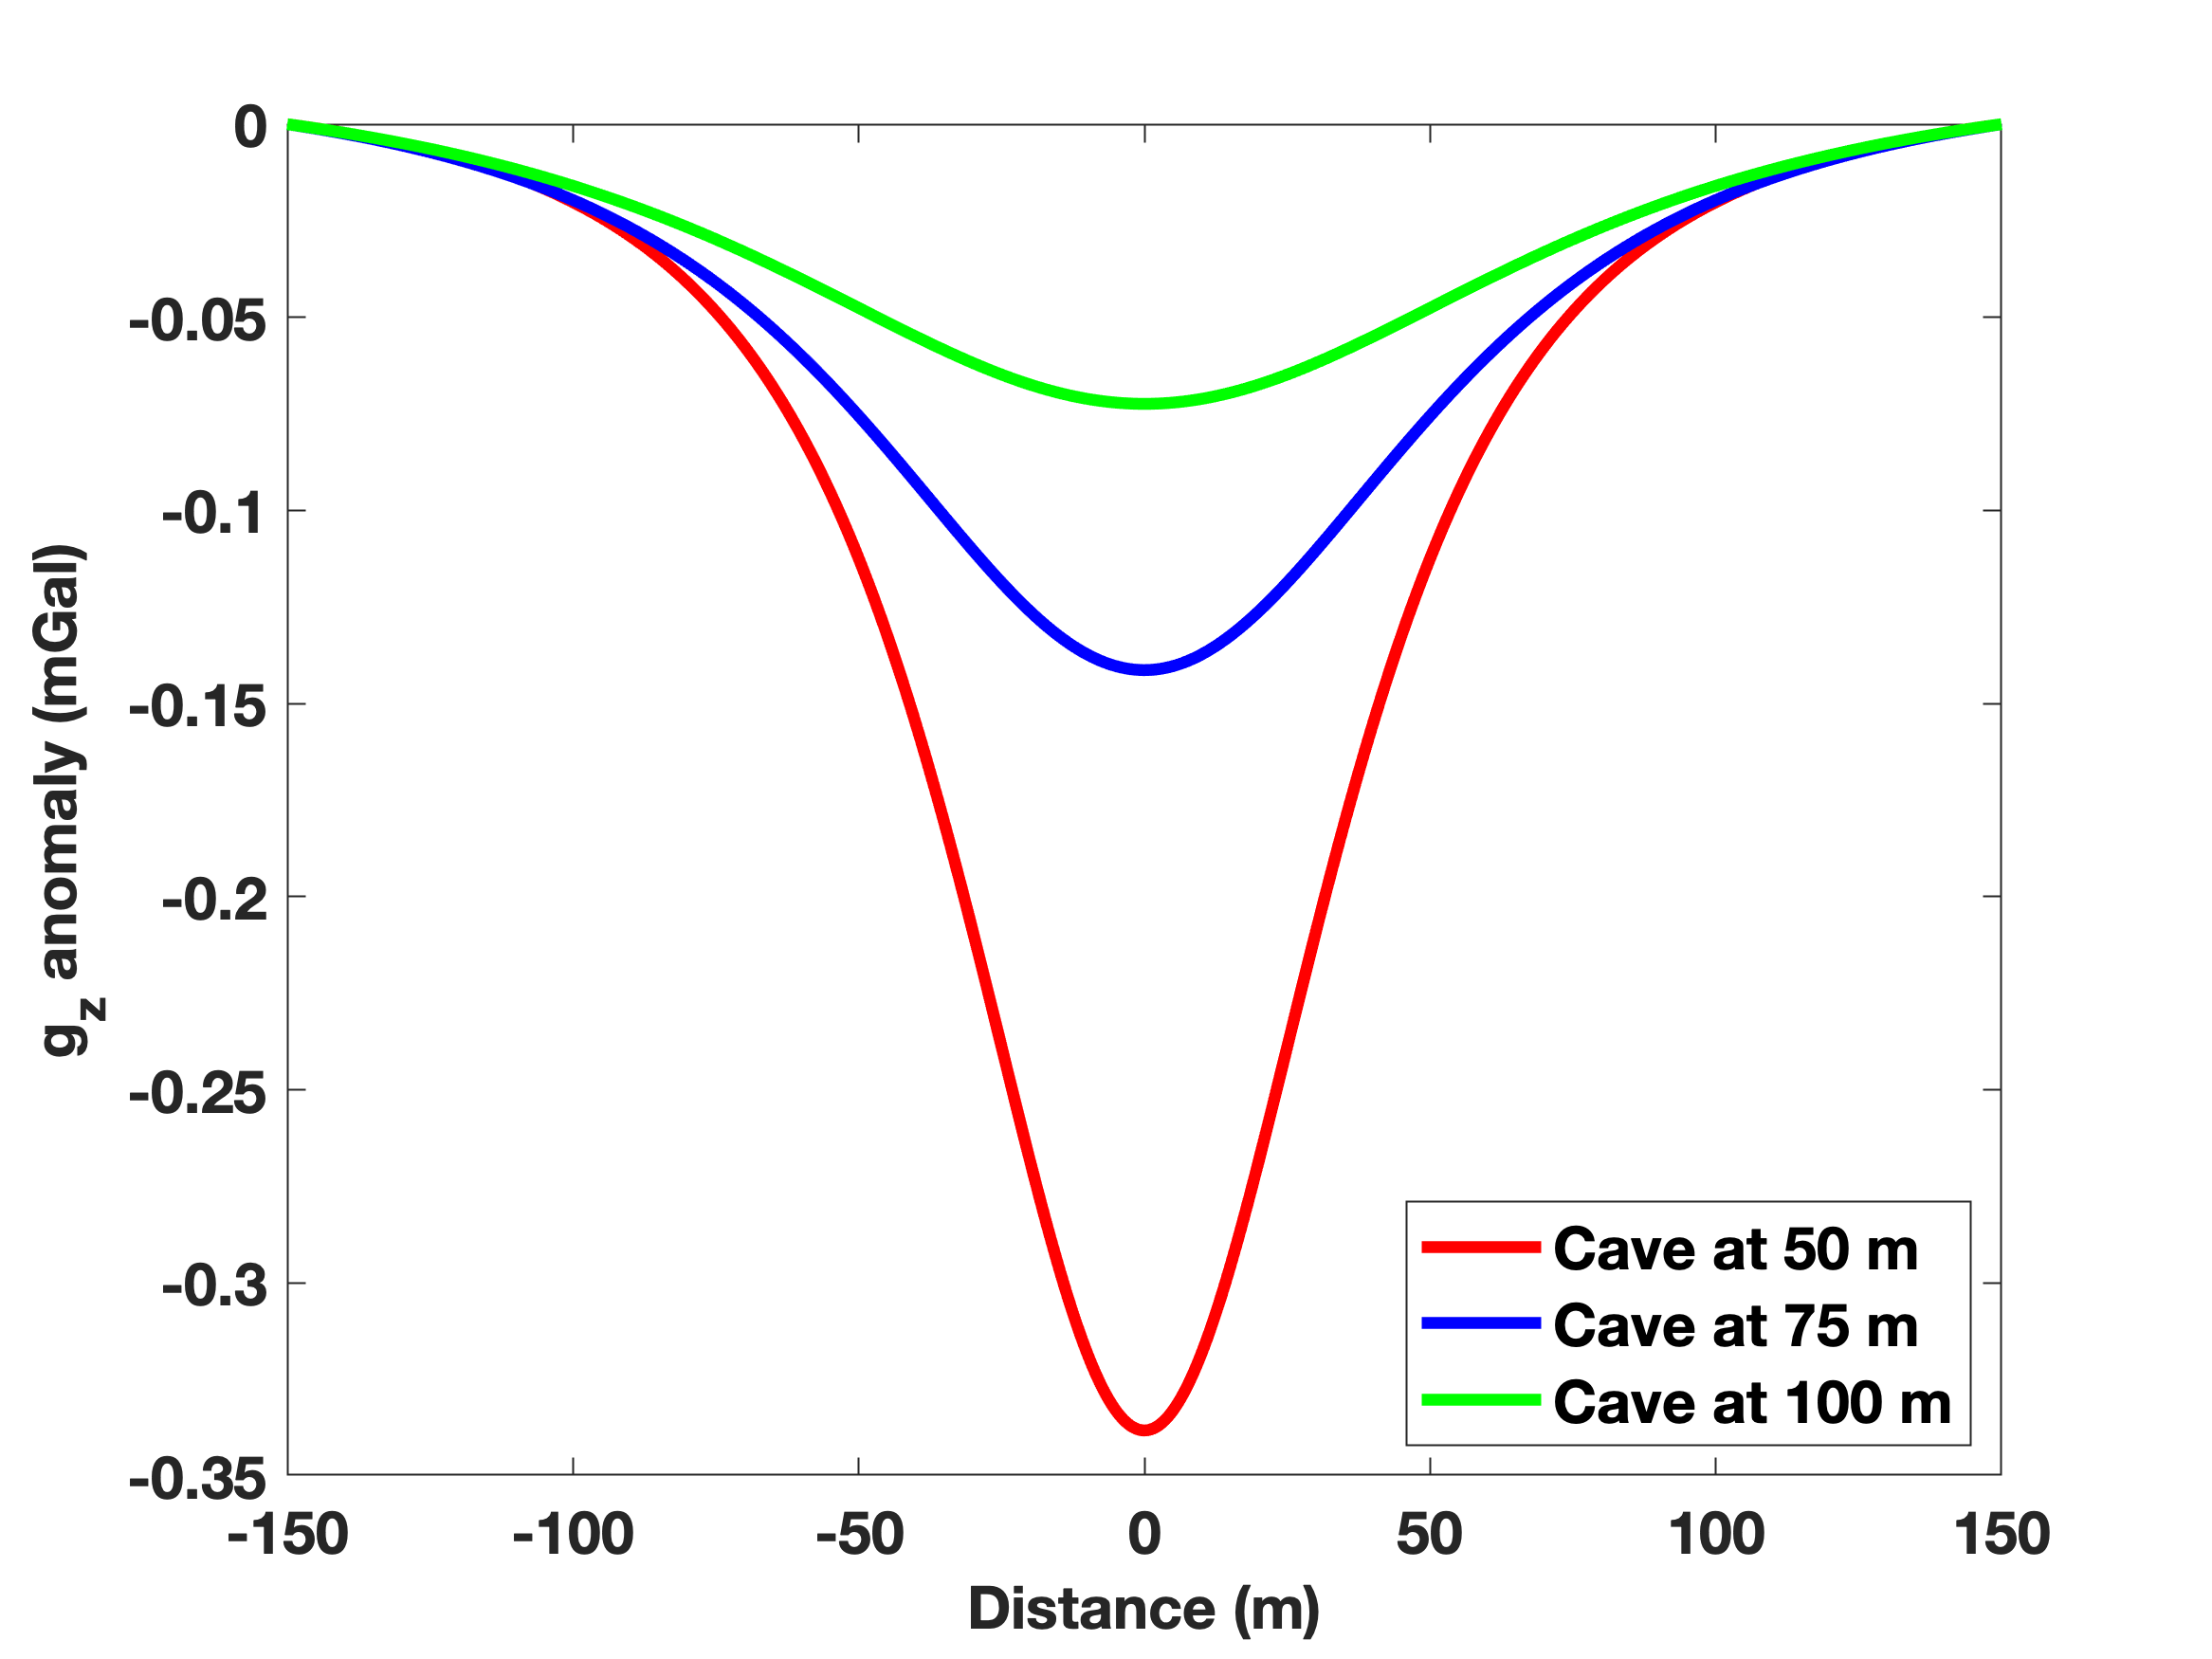
\includegraphics[width=0.5\textwidth]{Figures/Gravimetry/Gravimetry01_Visualization.png}
    \end{center}
 
    \textbf{(d)}This requires some arithmetic manipulation to isolate $z$.
\begin{eqnarray*}
g_z &=\frac{1}{2}g_{z,max} \\
\rightarrow \frac{z}{(x^2_{1/2}+z^2)^\frac{3}{2}} &= \frac{1}{2z^2}\\
\rightarrow \frac{z^3}{(x_{\frac{1}{2}}+z^2)^\frac{3}{2}}&= \frac{1}{2}\\
\rightarrow \frac{1}{(\frac{x_{\frac{1}{2}}}{z^2}+1)^\frac{3}{2}}&= \frac{1}{2}\\
\rightarrow z = \frac{x_{1/2}}{\sqrt{2^{\frac{2}{3}}-1}}\approx 1.305 x_{1/2}
\end{eqnarray*}
Those expressions can be useful to estimate the depth of an object from an observed anomaly without using a full forward model. However, this only works if the object is close to spherical (which we usually don't know necessarily ahead of time.) Similar estimates exists for other shapes (e.g., horizontal and vertical cylinders).
\end{tcolorbox}
\fi